\section{Natural Language Processing}
\label{sect:natural-language-processing}
NN applications in NLP
\begin{itemize}
	\item Classification/Sequence labeling problems
	\item Language Modeling and Word Embeddings
	\item Sentence Modeling
	\item Machine Translation
	\item Dialog Systems
\end{itemize}
Tasks Of NLP:
\begin{itemize}
	\item Part-Of-Speech: label each word
	\item Chunking: label segments of a sentence (noun or verb phrase)
	\item Named Entity Recognition: label atomic elements (person, locatin)
	\item Semantic Role Labeling: label elements of a sentence with a semantic role 
\end{itemize}
\textbf{Window of n-gram}: $k$ words before, $k$ words after currentl 
considering word: $n= 2*k + 1$
\textbf{1-of-N coding(one-hot)}: a vocabulary-size-dimensional vector, 1 in the index of the word, 0 otherwise.

\subsection{Language Model}
\label{ssect:language-model}
Model how fluent a sentence is. Given sentence S, calculate P(S). Given incomplete sentence H, calculate P(wordX | H).Probability of the next word given a history (MLE):
\[
P(w_i|H) = P(w_i | w_1 ... w_{i-1}) = \frac{count(w_1 ... w_i)}{count(w_1 ... w_{i-1})}
\]
Conventional n-gram approach (only n previous words):
\[
P(w_i|H) \approx P(w_i | w_{i-n+1} ... w_{i-1}) = \frac{count(w_1 ... w_i)}{count(w_{i-n+1} ... w_{i-1})}
\]
Probability of the whole sentence S:
\[
P(S) = P(w_1 ... w_N) \approx \Pi_{i=1}^N P(w_i | w_{i-n+1} ... w_{i-1})
\]
\begin{figure}[h]
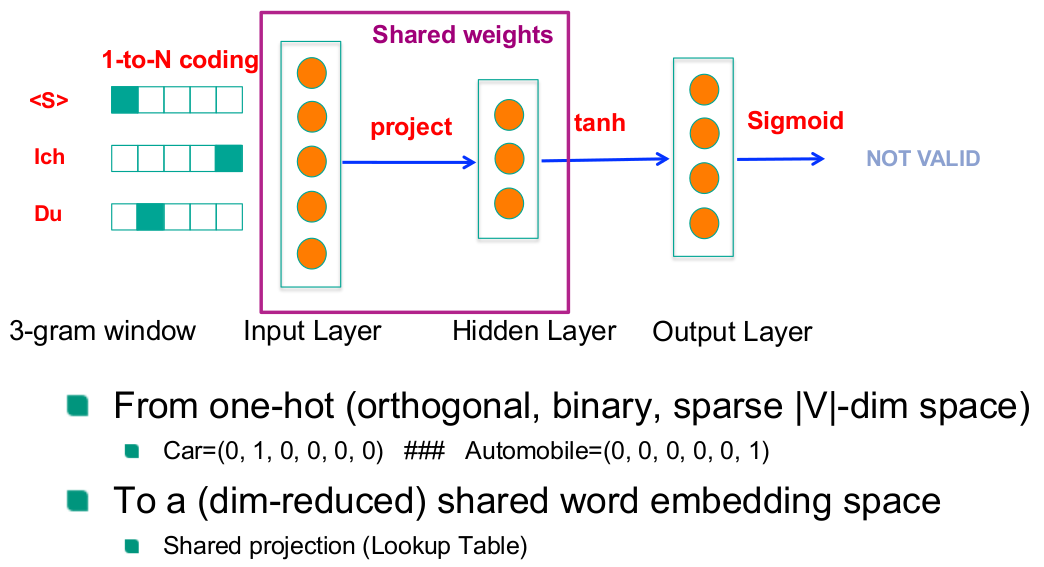
\includegraphics[scale=0.4]{word-embeddings}
\end{figure}
\subsubsection{Word Embeddings}
\label{sssect:word-embeddings}
Spatial distance corresponds to word similarity: we(car) close to we(automobile).\\
Vector operations can be used to combine word meanings: we(king)-we(queen) ~ we(man)-we(woman)

\subsubsection{Word2Vec}
needed??

\subsection{Sentence Modeling}
\label{ssect:sentence-modeling}
Representation of word sequences: Need fixed-length representation vectors for variable-length sequences.\\
Approaches:
\begin{itemize}
	\item Simple aggregation: Sum/Average/Max?
	\item Recurrent architectures: One word vector at a time step
	\item Recursive NN: Compositions using syntax parsed tree
	\item Time-Delay NN or Convolutional NN
\end{itemize}
Convolutional:\\
input sequence: $\mathbf{s} \in \mathbf{R}^s$\\
Filter vector: $\mathbf{m} \in \mathbf{R}^m$ (??????)\\
Take the dot product from $\mathbf{m}$ with each m-gram in $\mathbf{s}$ to obtain a sequence $\mathbf{c_j}$:
\[
\mathbf{c_j} = \mathbf{m}^T \cdot \mathbf{s}_{j-m+1:j}
\]
After convolution step we have a matrix $\mathbf{c_j}$ (sequence of vectors) but still be a variable-length sequence (on $s$): $\mathbf{c}_j \in \mathbf{R}^{m x s}$\\
Max Pooling: Take the max value of each row in $\mathbf{c_j}$ . Now we have a fixed-length vector (on $m$).\\
Exactly the same as Time-Delay Neural Networks (TDNN)

\subsubsection{Dynamic k-max Convolutional NN}
\label{sssect:dcnn}
\begin{figure}[h]
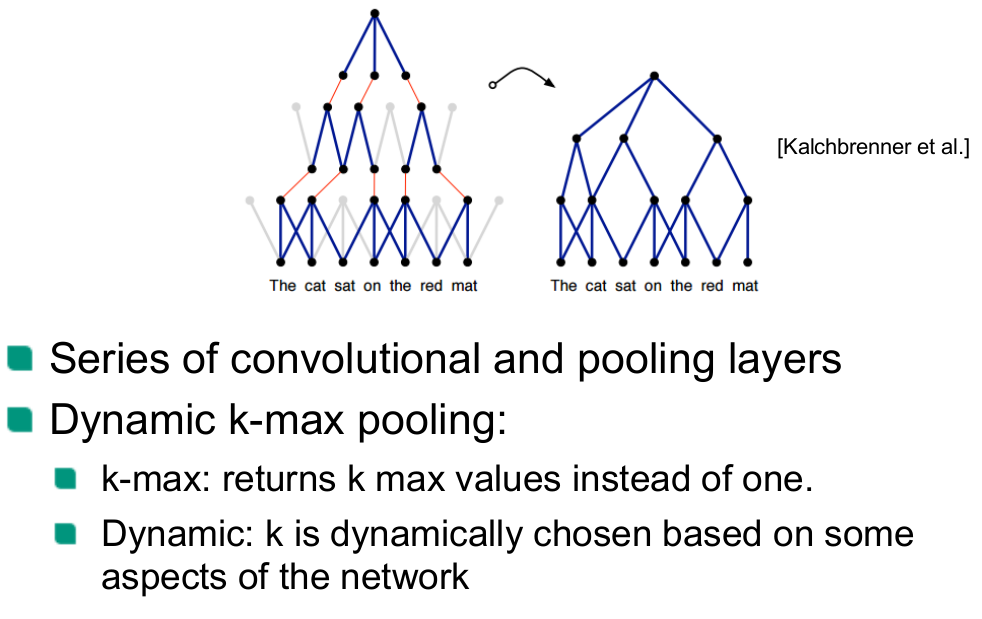
\includegraphics[scale=0.4]{DCNN}
\end{figure}
Advantages
\begin{itemize}
\item A filter is a linguistic feature detector of a class of n-grams
\item Features are extracted independently from their positions.
\item Higher filters can capture syntactic and semantic info.
\end{itemize}
Dynamic k-max pooling:
\[
k_I = max(k_{top}, \lceil \frac{L - I}{L} S \rceil)
\]
$k_{top}$: fixed $k_{top}$ pooling layer on top\\
$I, L$: convolutional layer $I$ over total $L$ convolutional layers where the $k^{th}$ applied on.\\
Properties:
\begin{itemize}
\item Sensitivity to word and n-gram order
\item Have the ability to induce feature graph
\end{itemize}
\newpage